\documentclass[a4paper]{article}
\usepackage{graphicx}
\usepackage{mathtools}
\usepackage{listings}
\usepackage{wasysym}
\usepackage{color}
\usepackage[margin=1in]{geometry}
\DeclareGraphicsExtensions{.png}
\lstset{language=SQL,
    basicstyle=\ttfamily,
    breaklines=true,
    keywordstyle=\color{blue}\ttfamily,
    stringstyle=\color{red}\ttfamily,
    commentstyle=\color{green}\ttfamily,
    morecomment=[l][\color{magenta}]{\#}
}

\setcounter{secnumdepth}{2}
\begin{document}

\title{Coursework 1: Databases}
\author{Liban Abdulkadir}

\maketitle

\section*{Question A}
\begin{enumerate}
    \item $ \pi_{Title} (Module) $
    \item $ \pi_{Name} (\sigma_{Year = 1}(Student)) $
    \item $ \pi_{MID} (Enrolment) $ \\ \\
            There may be several $Enrolment$ records with the same $MID$,
            however the default behaviour of $\pi_{A} (R)$ is to return
            unique $A$ entries.
    \item $ \pi_{MID} (Module) - \pi_{MID} (Enrolment) $ \\ \\
            The right operand relation refers to the list of $MID$s that
            have 1 or more students enrolled on the respective module.
            Subtracting this result from the list of all modules in
            existence using the difference operator gives us the opposite,
            which is modules with 0 students.
    \item $ R_1 = \pi_{MID} (Module) - \pi_{MID} (Enrolment) $ \\
          $ \pi_{Title} (Module \Join R_1) $ \\ \\
            $R_1$ is the relation giving $MID$s of modules with no
            students from the previous question. The natural join
            operation allows us to get the values of all attributes of
            $Module$ for $R_1$. Projection is then used to obtain only
            the list of $Title$s.
    \item $ R_1 = (Student \times Module) $ \\ \\
          $ R_2 = R_1 \Join Enrolment $ \\ \\
          $ R_3 = \pi_{Name,Title} (R_2) $ \\ \\
          $ \rho_{R_3(StudentName,ModuleTitle)} (R_3) $ \\ \\
            Relation $R_1$ describes all possible $Student$-$Module$ 
            combinations. 
            The schema for this relation contains $Name$ and 
            $Title$ (among others).
            After performing a natural join on $R_1$ and Enrolment, whose 
            common attributes are $SID$ and $MID$,   
            only combinations such that $R_1.MID = Enrolment.MID 
            \cap R_1.SID = Enrolment.SID$ remain. This gives us names of 
            students and titles of modules they are enrolled on 
            where $Name$ and $Title$ may appear more than once. Projection 
            is then used to retain only student names ($Name$) and module 
            titles ($Title$). Finally, we rename the attributes of the 
            previous result to be more descriptive.   
    \item $ R_1 = \sigma_{Year = 3}(Student) 
            \times \sigma_{Department = 'Computer Science'}(Module) $ \\ \\
      $ R_2 = R_1 \Join Enrolment $ \\ \\
      $ R_3 = \pi_{Name} (R_2) $ \\ \\
            Cartesian product is used to obtain a relation representing all
            possible $Student$-$Module$ combinations where every student is Year 3
            and every module belongs to the Computer Science department.
            Similarly to the previous question, natural join is used to constrain
            all potential $Student$-$Module$ combinations to those that are valid
            (i.e. the student is enrolled on that module). Next, projection is used
            to obtain just the student names.
    \item $ R_1 = Student 
            \times \sigma_{Title = 'Databases' \vee Title = 'Concurrency' }(Module) $ \\ \\
      $ R_2 = R_1 \Join Enrolment $ \\ \\
      $ R_3 = \pi_{SID} (R_2) $ \\ \\
            The condition in the selection operator ensures that only modules with titles
            'Databases' or 'Concurrency' will be used later in the natural join, meaning
            $Enrolment$ records with $MID$s corresponding to other modules will not be 
            selected.
    \item $ TS = \pi_{SID,Assignment + Exam} ((\sigma_{Title = 'Databases'} Module) \Join Enrolment) $ \\ \\
        $  TS_1 = \rho_{TS_1(SID,Total)} (TS) $ \\ \\
        $  TS_2 = \rho_{TS_2(SID,Total)} (TS) $ \\ \\
        $  TSS = \sigma_{TS_1.Total < TS_2.Total} (TS_1 \times TS_2) $ \\ \\
        $  NO\_MAX = \rho_{NO\_MAX(SID,Total)} (\pi_{TS_1.SID,TS_1.Total} (TSS)) $ \\ \\
        $  ONLY\_MAX = TS_1 - NO\_MAX $ \\ \\
        $  MAX\_NAMES = \pi_{Name} (ONLY\_MAX \Join Student) $ \\ \\
        $TS$ represents $SID$s and total $Assignment$ and $Exam$ mark for all students 
        enrolled on the 'Databases' module.
        The renaming operator is used to correctly perform the product of TS with itself.
        All records for which $TS_1.Total < TS_2.Total$ are then excluded, which implies that
        $TS_1.Total$ will never be equal to the MAX of $Total$. \\
        $TS_1.SID$ and $TS_1.Total$ are then projected to become $NO\_MAX$. At this point 
        $NO\_MAX$ has an identical schema to $TS_1$ and $TS_2$ and does not contain the maximum (s)
        so the difference operator is used to obtain the record with just the maximum (s). \\
        Similarly to previous questions, the names corresponding to $SID$s in $ONLY\_MAX$ 
        are obtained by performing natural join with $Student$ and then projection to keep
        just the names.
    \item $ AVGS = MID \mathcal{F}_{average(Assignment + Exam)\; as\; avgtotal} (Enrolment) $ \\ \\
        $ E\_AVGS = Enrolment \Join AVGS $ \\ \\
        $ LOW\_SIDMIDS = \pi_{SID,MID} (\sigma_{Assignment + Exam < 0.4*avgtotal} (E\_AVGS)) $ \\ \\
        $ NAME\_MIDS = \pi_{Name,MID} ((\sigma_{Year = 3} Student) \Join LOW\_SIDMIDS ) $ \\ \\
        $ NAME\_TITLES = \pi_{Name,Title} (NAME\_MIDS \Join Module) $ \\ \\
        First, the average total mark for every module is calculated. This is done using the $average$
        aggregate function with grouping by attribute $MID$. $AVGS$ has 2 attributes - $MID$ and $avgtotal$.
        $E\_AVGS$ is $Enrolment$ with the total mark average added corresponding to $MID$s by joining $AVGS$.
        $ LOW\_SIDMIDS $ gives us student IDs and corresponding module IDs from the enrolment table where
        the total ($Assignment + Exam$) mark is less than 40\% of the average mark for that module.\\
        Next we use natural join to restrict the result to Year 3 students and add $Name$ to the schema. 
        Projection is then used to keep only $Name$ and $MID$. The result is then joined with $Module$ 
        allowing us to obtain module titles given $MID$s.
\end{enumerate}

\section*{Question B}
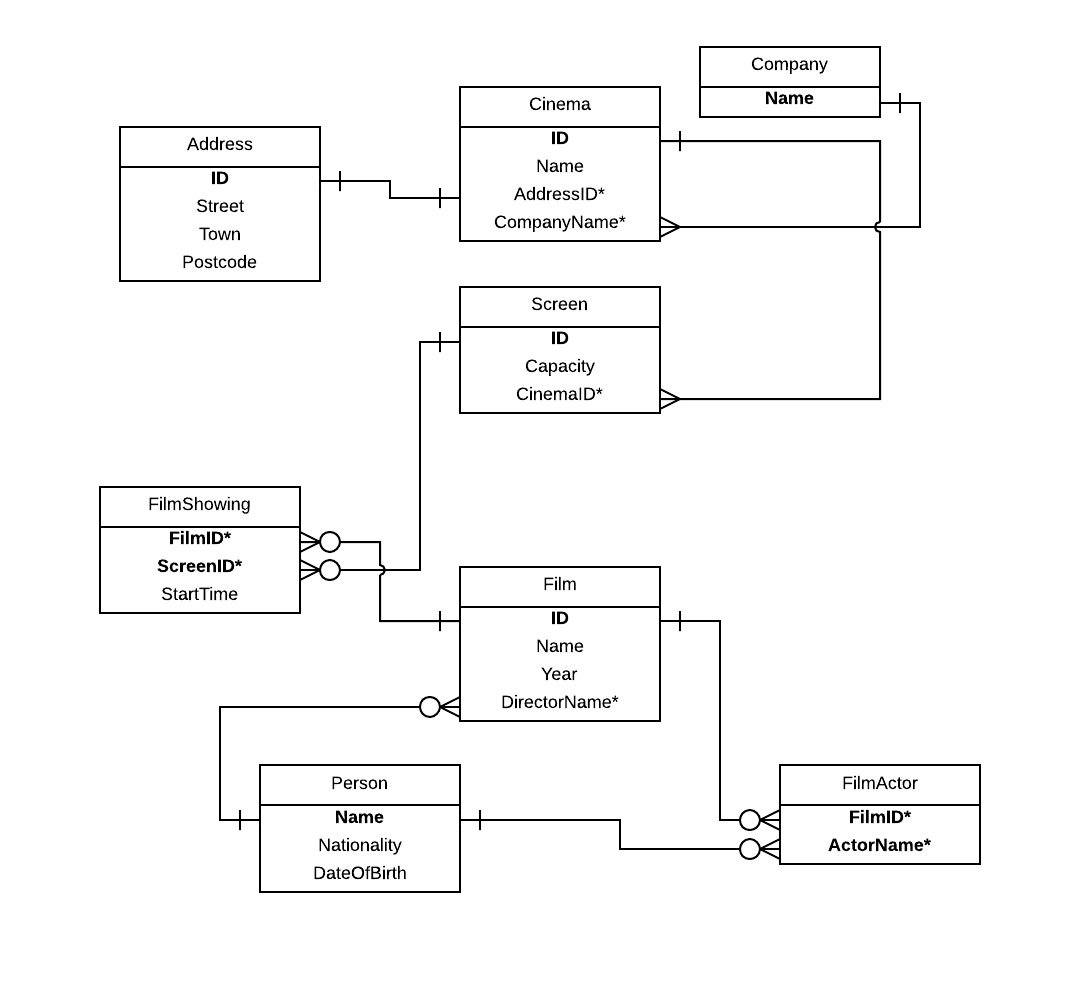
\includegraphics[scale=0.5]{erd}\newline
Primary keys are shown in \textbf{bold}. Foreign keys are marked with asterisks (*).
Attributes that are both bold and marked with asterisks are compound keys (in entities $FilmShowing$ and $FilmActor$).
\section*{Question C}
\lstinputlisting[language=SQL]{cw.sql}
\end{document}
